%%%%%%%%%%%%%%%%%%%%%%%%%%%%%%%%%%%%%%%%%%%%%%%%%%%%%%%%%%
%% BEGIN PREAMBLE
\documentclass[10pt]{article}

%%%% Sets 1 inch margins on document
\usepackage[margin=1in]{geometry}

%%%% For math macros
\usepackage{amsmath}

%%%% Needed for including figures and other images
\usepackage{graphicx}

%%%% Adds ability to adjust document vertical spacing
% usage:
%   \setspace{1.5} % 1.5x for line spacing
\usepackage{setspace}

%%%% Needed for specifying the list items in enumerate env
% eg. (a,b,b) or (i,ii,iii), (1,2,3)
% usage:
%   \begin{enumerate} [label=(\alph*)] % for (a), (b), (c)
\usepackage{enumitem}

%%%% Defines Times New Roman as font
  % for math and text environments
\usepackage{newtxtext,newtxmath}

%%%% For H float option when inserting figure
%   [H] inserts figure _exactly_ where it is typeset
% usage:
%   begin{figure} [H]
\usepackage{float}

%%%% For fancy header and footer ;)
\usepackage{fancyhdr}
\pagestyle{fancy}
\fancyhead[LO,L]{Samuel Barton}
\fancyhead[CO,C]{ENGS31 - Lab 5}
\fancyhead[RO,R]{\today}
\fancyfoot[LO,L]{}
\fancyfoot[CO,C]{\thepage}
\fancyfoot[RO,R]{}
\renewcommand{\headrulewidth}{0.4pt}
\renewcommand{\footrulewidth}{0.4pt}

%%%% Setting margins in tabular environments
% For making equations (esp. fractions) fit in cells vertically
\usepackage{cellspace}
\cellspacetoplimit 4pt
\cellspacebottomlimit 4pt
%% END PREAMBLE %%
%%%%%%%%%%%%%%%%%%%%%%%%%%%%%%%%%%%%%%%%%%%%%%%%%%%%%%%%%%%%%%%

\begin{document}

\setstretch{1.25} % set spacing to 1.25x

% Assignment Name
\begin{centering}
  \section*{LAB 5}
\end{centering}

\subsection*{Deliverable 1: Block Diagram}

\begin{figure} [H]
  \center
  \includegraphics[width=0.95\textwidth]{figures/block_diagram.png}
  \caption{Block Diagram}
\end{figure}

\subsection*{Deliverable 2: Datapath RTL Model and VHDL}

See VHDL file attached separately...

\begin{figure} [H]
  \center
  \includegraphics[width=0.95\textwidth]{figures/datapath.png}
  \caption{Datapath RTL Diagram}
\end{figure}

\subsection*{Deliverable 3: State Machine}

See VHDL file attached separately...

\begin{figure} [H]
  \center
  \includegraphics[width=0.95\textwidth]{figures/FSM.png}
  \caption{Finite State Machine for the Controller}
\end{figure}

\subsection*{Deliverable 4: Clock Divider}
\[
  TC := 50
\]

\subsection*{Deliverable 5: Controller Test Bench}

\subsubsection{Planned Tests}
\begin{enumerate}
  \item Normal Operation
  \item Clear on sB state (premature clear)
  \item Hold Clear and try to load number
\end{enumerate}

\subsubsection{Testbench Code}
See VHDL file attached separately...

\subsubsection{Annotated Testbench Waveform}

\begin{figure} [H]
  \center
  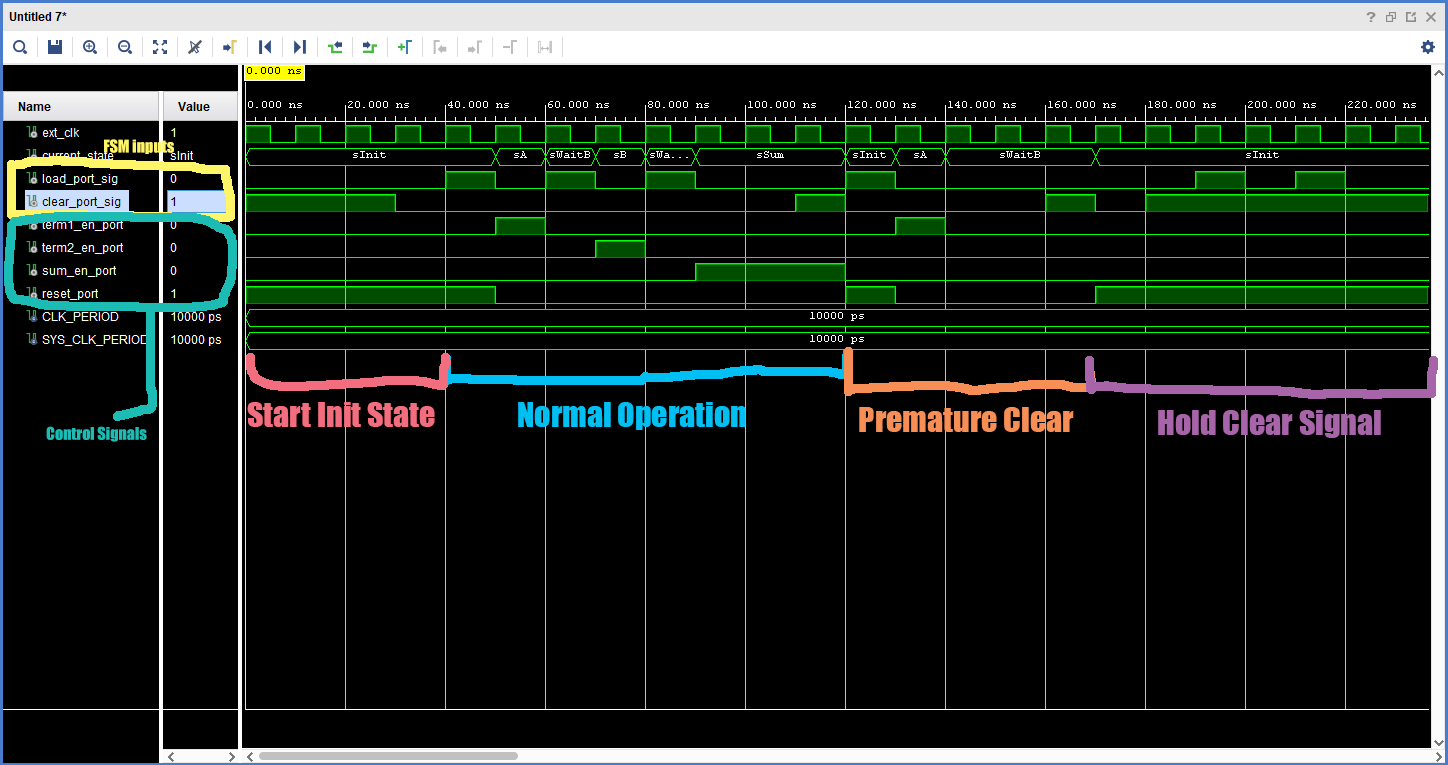
\includegraphics[width=0.95\textwidth]{figures/controllor_tb_wav_annotated.png}
  \caption{Annotated Controller Testbench Waveform, Annotated (Note How Control Signals Follow the FSM)}
\end{figure}

\begin{figure} [H]
  \center
  \includegraphics[width=0.45\textwidth]{figures/testbench_sig.png}
  \caption{Staff Signature for Controller Test Bench}
\end{figure}

\subsection*{Deliverable 6: Elaborated Schematic}

\begin{figure} [H]
  \center
  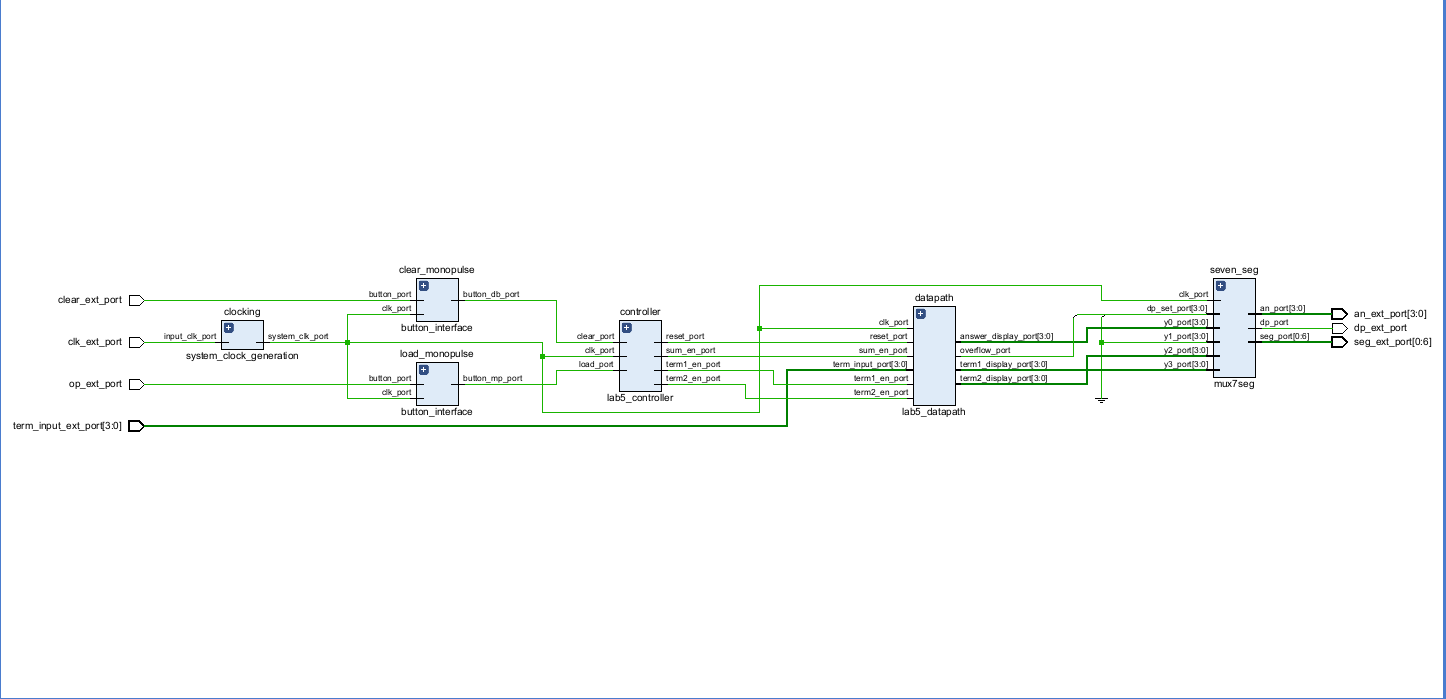
\includegraphics[width=0.95\textwidth]{figures/full_rtl.png}
  \caption{Full RTL Schematic}
\end{figure}

\begin{figure} [H]
  \center
  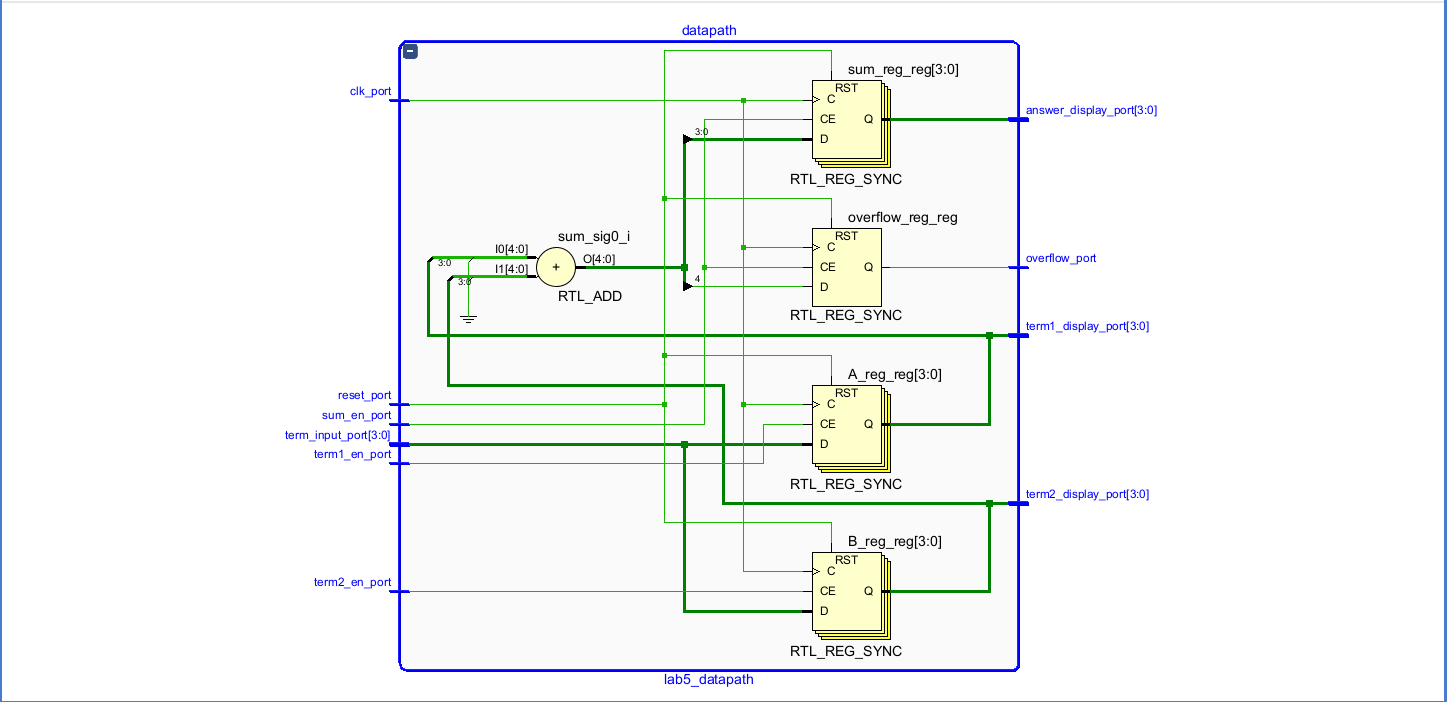
\includegraphics[width=0.65\textwidth]{figures/datapath_rtl.png}
  \caption{Datapath RTL Schematic}
\end{figure}

\subsection*{Deliverable 7: Top Level Testbench}

\begin{figure} [H]
  \center
  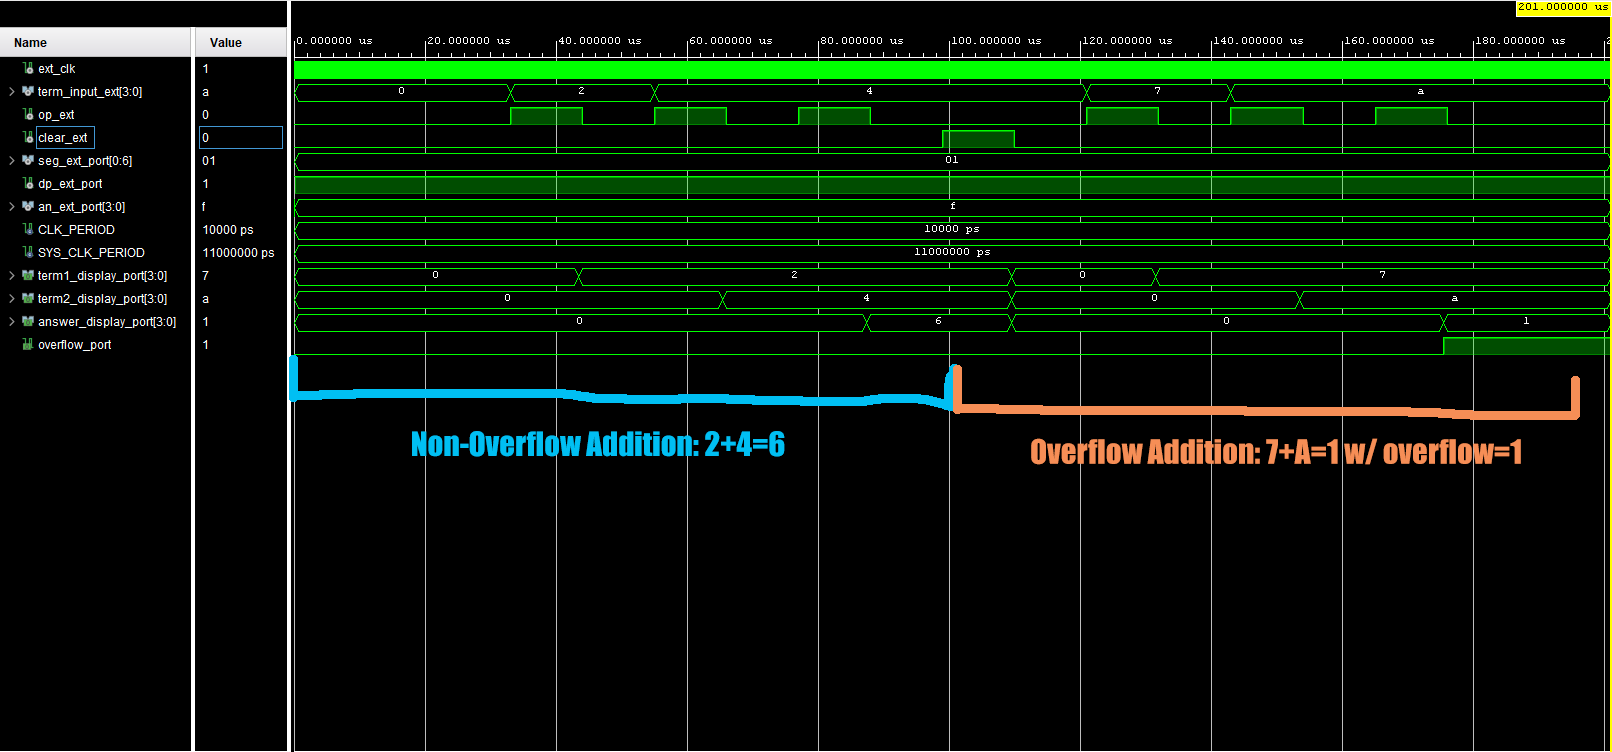
\includegraphics[width=0.95\textwidth]{figures/shell_tb_annotated.png}
  \caption{Top Level Simulation Waveform, Annotated}
\end{figure}

\subsection*{Deliverable 8: Program Your FPGA}

\begin{figure} [H]
  \center
  \includegraphics[width=0.65\textwidth]{figures/hw_val_sig.png}
  \caption{Staff Signature for Hardware}
\end{figure}

\subsection*{Deliverable 9: Reflections}
For me, the most difficult steps of the process were designing the FSM and writing the timing logic for the testbenches.

For the FSM, I initially didn't include the waiting states between loading the numbers and displaying the sums which would not have been per spec.
However, this ended up being a quick fix because I just had to add those intermediate states.
Another bug that I discovered was that I used the output pin, reset\_signal, interchangeably with the input port, clear\_port, since they had similar names.
This slight error led to difficult to find errors in the elaboration step. 
The most difficult step was writing the testbench for the controller.
Initially, I was not monopulsing the button inputs which led to unexpected behavior with the FSM states.
Once realizing this however, I had to make sure to sync these button presses with the clock period.
Once writing the testbench for the full design, I also had to take in account the slower clock pulse from the clock divider, which in turn, complicated the timing.

\end{document}

